\section{Ανάλυση Fourier}
    \subsubsection{Περιοδικές συναρτήσεις με περίοδο $T$}
    \begin{gather*}  
    x_k =\sqrt{\frac{2}{T}} \cos(k\omega t)\qquad \omega = \frac{2\pi}{T}
    \text{ θεμελιώδης κυκλική συχνότητα}
    \\
    \left\langle 
    x_k(t),x_n(t)
    \right\rangle =
    \int_{-\sfrac{T}{2}}^{\sfrac{T}{2}} x_k(t)x_n(t)\dif t
    = \int_{-\sfrac{T}{2}}^{\sfrac{T}{2}} \cos(k\omega t)\cos(n\omega t)\dif t
    = \begin{cases}
    n \neq k \to 0 \\ n = k \to 1
    \end{cases}
    \end{gather*}
    \begin{gather*}
        y_k = \sqrt{\frac{2}{T}}\sin(k\omega t)
        \left\langle
        y_k,y_n
        \right\rangle = \begin{cases}
        n \neq k \to 0 \\ n = k \to 1
        \end{cases}
    \end{gather*}
    
    Υποστηρίζω ότι κάθε περιοδική \( \displaystyle 
    f(t) = \sum_{n=0}^\infty a_n\cos(n\omega t)+b_n\sin(n\omega t) \)
    
    Οραματίζομαι ότι αν η παραπάνω \( f(t) \) είναι σήμα εισόδου σε ένα σύστημα,
    τα ημίτονα και συνημίτονα ως ιδιοσυναρτήσεις θα παραμείνουν αμετάβλητα,
    και θα τροποποιηθούν μόνο τα \( a_n, b_n \).
    
    \begin{gather*}
    z_k(t) =  e^{jk\omega t} \\
    \left\langle
    z_k,z_n
    \right\rangle = \begin{cases}
    k\neq n \to 0 \\
    k = n \to T
    \end{cases}\\
    z_k(t)=\frac{1}{\sqrt{T}}e^{jk\omega t}
    \end{gather*}
    
    \begin{gather*}
    \boxed{
    f(t) = \sum_{n=-\infty}^\infty F_n e^{jn\omega t}
    } \text{ εκθετική σειρά} \\
    \boxed{
        f(t) =\frac{a_0}{2} + \sum_{n=1}^\infty \left[
        a_n\cos(n\omega t)+b_n\sin(n\omega t)
        \right]
        } \text{ τριγωνομετρική σειρά Α} \\
    \boxed {
        f(t) = A_0 + \sum_{n=1}^\infty A_n\cos(n\omega t+\phi_n)
        } \text{ τριγωνομετρική σειρά Β}
    \end{gather*}
    
    Οι συντελεστές μπορούν να βρεθούν από τις προβολές της συνάρτησης πάνω στα
    ημίτονα και τα συνημίτονα:
    \begin{align*}
    a_n &= \frac{2}{T} \int_{-\sfrac{T}{2}}^{\sfrac{T}{2}} f(t)\cos(n\omega t)\dif t
    \quad n \neq 0 \\
    b_n &= \frac{2}{T} \int_{-\sfrac{T}{2}}^{\sfrac{T}{2}} f(t)\sin(n\omega t)\dif t
    \\ a_0 &= \frac{2}{T} \int_{-\sfrac{T}{2}}^{\sfrac{T}{2}} f(t)\dif t
    \\[5pt] F_n &= \frac{1}{T} \int_{-\sfrac{T}{2}}^{\sfrac{T}{2}}
    f(t)e^{-jn\omega t}\dif t
    \end{align*}
    
    \paragraph{Συνθήκες Dirichlet}
    \begin{enumpar}
        \item \( 
        \displaystyle \int_{-\sfrac{T}{2} }^{\sfrac{T}{2} }\left|
        f(t)
        \right| \dif t < \infty
         \)
        \item Πεπερασμένο πλήθος ασυνεχειών εντός \( T \)
        \item Πεπερασμένος αριθμός τοπικών ακροτάτων εντός \( T \)
    \end{enumpar}
    
    \( f(t) \) περιοδική \( T \)
    
    \hspace{-2cm}
    \begin{tabular}{|c|c|c|c|}
        \hline \textbf{Μορφή} & \textbf{Σειρά}  & \textbf{Συντελεστές} & \textbf{Αλλαγές} \\ 
        \hline Εκθετική & \(\displaystyle f(t)=\sum_{-\infty}^\infty F_n e^{j\omega n t} \) &
        \(\displaystyle F_n = \frac{1}{T} \int_{-\sfrac{T}{2}}^{\sfrac{T}{2}}
        f(t)e^{-jn\omega t}\dif t\) &\(
        \begin{array}{l}
            F_0 = \sfrac{a_0}{2} \\ F_n = \sfrac{1}{2} (a_n-jb_n)  
        \end{array}\)
         \\ 
        \hline {\small Τριγωνομετρική} Α  & \( 
        \displaystyle f(t)=\frac{a_0}{2}+\sum_{n=1}^\infty a_n\cos(n\omega t)
        +b_n\sin(n\omega t)
         \)  & \(
         \begin{array}{ll}
         a_n &= \frac{2}{T} \int_{-\sfrac{T}{2}}^{\sfrac{T}{2}} f(t)\cos(n\omega t)\dif t \\
         b_n &= \frac{2}{T} \int_{-\sfrac{T}{2}}^{\sfrac{T}{2}} f(t)\sin(n\omega t)\dif t \\ a_0 &= \frac{2}{T} \int_{-\sfrac{T}{2}}^{\sfrac{T}{2}} f(t)\dif t
         \end{array}
         \) & 
         \(
         \begin{array}{l}
         a_n = (F_n+F_{-n})\\
         b_n=j(F_n-F_{-n})\\
         a_0=2F_0
         \end{array}
         \)
         \\ 
        \hline 
        {\small Τριγωνομετρική} Β
        & \(
        f(t) = A_0 + \sum_{n=1}^\infty A_n\cos(n\omega t+\phi_n)
        \) & &
        \(
        \begin{array}{l}
        A_0 = \sfrac{a_0}{2} \\
        A_n = \sqrt{a_n^2+b_n^2} = 2|F_n| \\
        \phi_n = \arctan\left(\frac{b_n}{a_n}\right)
        \end{array}
        \)
        \\ \hline
    \end{tabular} 
    
    \paragraph{}
    \begin{align*}
    P &= \frac{W}{T} = \frac{1}{T} \int_0^T f^2(t)\dif t =  
    \frac{a_0^2}{4}+\frac{1}{2}\sum_{n=1}^\infty a_n^2+b_n^2
    \\ &= F_0^2+2\sum_{n=1}^\infty |F_n|^2 = 
    \sum_{n=-\infty}^\infty \left|F_n\right|^2 
    \end{align*}
    
    \paragraph{Άσκηση για το σπίτι}
    Να βρεθούν η εκθετική και η τριγωνομετρική σειρά των σημάτων:
    
    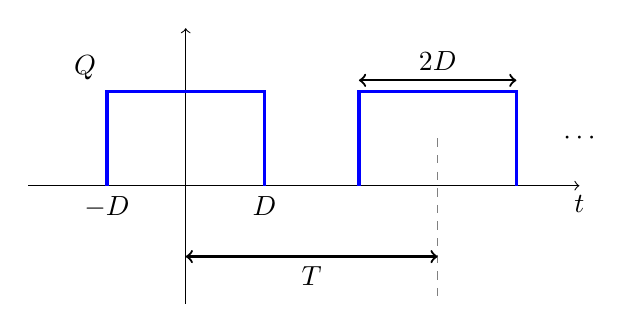
\begin{tikzpicture}
    \draw[->] (0,-1.5) -- (0,2);
    \draw[->] (-2,0) -- (5,0) node[below] {$t$};
    
    \draw[very thick,draw=blue]
    (-1,0) node[below] {$-D$} -- ++(0,1.2) node[above left] {$Q$} 
    -- ++(2,0) -- ++(0,-1.2) node[below] {$D$};
    
    \draw[very thick,draw=blue,xshift=3.2cm]
    (-1,0) -- ++(0,1.2) node[above left] (A) {}
    -- ++(2,0) node[above right] (B) {} -- ++(0,-1.2);
    
    \draw[thick,<->] (A) -- (B) node[midway,above] {$2D$};
    
    \draw (5,0.6) node {$\mathlarger{\mathlarger{\mathlarger{\cdots}}}$};
    
    \draw[dashed,gray] (3.2,0.6) -- ++(0,-2);
    \draw[thick,<->] (0,-0.9) -- ++(3.2,0) node[below,midway] {$T$};
    \end{tikzpicture}
    
    \begin{tikzpicture}
    \draw (0,-1.5) -- (0,2);
    \draw[->] (-2,0) -- (2,0) node[below] {$t$};
    
    \draw[very thick,blue] plot[variable=\x,samples=50,smooth,domain=-2:2]
    ({\x},{   abs(cos(pi/2*\x r))   });
    
    \draw[thick,<->] (-1,-0.2) -- ++(2,0) node[below right,midway] {$T$};
    
    \begin{scope}[xshift=5cm]
    \draw(0,-2) -- (0,2);
    \draw[->] (-1,0) -- (4,0) node[right] {$n$};
    
    \draw[ultra thick,orange!70!black] (0,0) -- ++(0,5/3);
    \draw[ultra thick,orange!70!black] (1,0) -- ++(0,4/3);
    \draw[ultra thick,orange!70!black] (2,0) -- ++(0,2/3);
    \draw[ultra thick,orange!70!black] (3,0) -- ++(0,-4/3);
    
    \filldraw (0,5/3) circle (1pt) node[left] {$Α_0$};
    \filldraw (1,4/3) circle (1pt) node[above] {$Α_1$};
    \filldraw (2,2/3) circle (1pt) node[above] {$Α_2$};
    \filldraw (3,-4/3) circle (1pt) node[left] {$Α_3$};
    
    \draw (0,0) node[below left] {$0$};
    \draw (1,0) node[below] {$1$};
    \draw (2,0) node[below] {$2$};
    \draw (3,0) node[above] {$3$};
    \end{scope}
    
    \begin{scope}[xshift=11cm]
    \draw(0,-2) -- (0,2);
    \draw (-1,0) -- (4,0);
    
    \draw[ultra thick,orange!60!black] (0,0) -- ++(0,5/3);
    \draw[ultra thick,orange!60!black] (1,0) -- ++(0,4/3);
    \draw[ultra thick,orange!60!black] (2,0) -- ++(0,2/3);
    \draw[ultra thick,orange!60!black] (3,0) -- ++(0,-4/3);
    
    \filldraw (0,5/3) circle (1pt);
    \filldraw (1,4/3) circle (1pt);
    \filldraw (2,2/3) circle (1pt);
    \filldraw (3,-4/3) circle (1pt);
    
    \draw (0,0) node[below left] {$0$};
    \draw (1,0) node[below] {$\frac{2\pi}{T}$};
    \draw (2,0) node[below] {$2\frac{2\pi}{T}$};
    \draw (3,0) node[above] {$3\frac{2\pi}{T}$};
    
    \draw[green!40!black,<->] (1,0.4) -- ++(1,0)
    node[midway,above] {$\frac{2\pi}{T}$};
    \end{scope}
    \end{tikzpicture}
    
    \subsection{Μετασχηματισμός Fourier}
    \begin{tikzpicture}[scale=1.2]
    \draw[->] (0,-1.5) -- (0,2);
    \draw[->] (-2,0) -- (2,0) node[below] {$t$};
    
    \draw[gray,dashed] (-1,1.8) -- ++(0,-3);
    \draw[gray,dashed] (1,1.8) -- ++(0,-3);
    
    \draw[very thick,blue] plot[smooth]
    coordinates {(-1,0) (-0.8,0.8) (-0.5,0.7) (0.3,1.5) (0.5,0.8) (0.7,0.75) (1,0)};
    \draw[xshift=-2cm,path fading=west,very thick,blue!60!cyan] plot[smooth]
    coordinates {(-1,0) (-0.8,0.8) (-0.5,0.7) (0.3,1.5) (0.5,0.8) (0.7,0.75) (1,0)};
    \draw[xshift=2cm,path fading=east,very thick,blue!60!cyan] plot[smooth]
    coordinates {(-1,0) (-0.8,0.8) (-0.5,0.7) (0.3,1.5) (0.5,0.8) (0.7,0.75) (1,0)};
    
    \draw (-1,0) node[below right] {$-\frac{T}{2}$};
    \draw (1,0) node[below right] {$\frac{T}{2}$};
    \end{tikzpicture}

    \paragraph{Φορέας} συνάρτησης είναι το διάστημα του πεδίου ορισμού της στο
    οποίο η συνάρτηση δεν είναι 0 (από \( \min x \) για το οποίο δεν είναι 0 ως
    το αντίστοιχο \( \max x \)).
    
    \begin{gather*}
    \tilde f(t) = \sum{k=-\infty}^\infty f(t-kT)\\
    \downarrow T\text{-περιοδική} \rightarrow \tilde f(t)=\frac{a_0}{2}
    +\sum_{n=1}^\infty a_n\cos(\omega_0 n t)+b_n\sin(\omega_0 n t)
    \qquad \omega_0=\frac{2\pi}{T} \\[3pt]
    f(t)=\begin{cases}
    \tilde f(t) &\quad -\sfrac{T}{2}\leq t \leq \sfrac{T}{2}\\
    0 &\quad\text{elsewhere} 
    \end{cases}
    \end{gather*}
    
    \begin{tikzpicture}
    \draw[->] (0,-2) -- (0,2) node[above] {$\mathrm{Term}(n)$};
    \draw[->] (-1,0) -- (5,0) node[right] {$n$};
    
    \draw[ultra thick,orange!70!black] (0,0) -- ++(0,2/3);
    \draw[ultra thick,orange!70!black] (1,0) -- ++(0,4/3);
    \draw[ultra thick,orange!70!black] (2,0) -- ++(0,-4/3);
    
    \filldraw (0,2/3) circle (1pt) node[left] {$\frac{a_0}{2}$};
    \filldraw (1,4/3) circle (1pt) node[above] {$a_1$};
    \filldraw (2,-4/3) circle (1pt) node[left] {$a_2$};
    
    \draw (0,0) node[below left] {$0$};
    \draw (1,0) node[below] {$1$};
    \draw (2,0) node[above] {$2$};
    
    \begin{scope}[yshift=-5cm]
    \draw[->] (0,-2) -- (0,2);
    \draw[->] (-1,0) -- (5,0) node[right] {$\omega$};
    
    \draw[ultra thick,orange!60!black] (0,0) -- ++(0,2/3);
    \draw[ultra thick,orange!60!black] (1,0) -- ++(0,4/3);
    \draw[ultra thick,orange!60!black] (2,0) -- ++(0,-4/3);
    
    \filldraw (0,2/3) circle (1pt) node[left] {$\frac{a_0}{2}$};
    \filldraw (1,4/3) circle (1pt) node[above] {$a_1$};
    \filldraw (2,-4/3) circle (1pt) node[left] {$a_2$};
    \filldraw (3,0) circle (1pt);
    
    \draw (0,0) node[below left] {$0$};
    \draw (1,0) node[below] {$\omega_0$};
    \draw (2,0) node[above] {$2\omega_0$};
    \draw (3,0) node[below] {$3\omega_0$};
    
    \draw[green!50!black,<->,thick] (0,0.4) -- ++(1,0)
    node[midway,above] {$\omega_0$};
    
    \draw (6,0) node[right] {$\omega_0 =\frac{2\pi}{T}$};
    \end{scope}
    \end{tikzpicture}
    
    \paragraph{Μετασχηματισμός Fourier}
    \begin{align*}
    F(\omega) &\overset{\triangle}{=}
    \int_{-\infty}^{\infty} f(t)e^{-j\omega t}\dif t
    \\ f(t) &= \frac{1}{2\pi}\int_{-\infty}^{\infty}
    F(\omega )e^{j\omega t}\dif\omega
    \end{align*}
    
    \begin{attnbox}{Προσοχή}
        Όταν παίρνουμε τύπους από τυπολόγια, ελέγχουμε τον ορισμό
        του μετασχηματισμού Fourier, για διαφορές στη σύμβαση!
    \end{attnbox}
    
    \paragraph{Αντίστοιχος ορισμός}
    \begin{align*}
    F(\mathfrak{f}) &\overset{\triangle}{=} \int_{-\infty}^{\infty}
    e^{-j2\pi\mathfrak{f}t}\dif t\\
    f(t) &= \int_{-\infty}^{\infty} F(\mathfrak f)e^{j2\pi\mathfrak{f}t}\dif
    \mathscr{f}
    \end{align*}
    (όπου \( \mathfrak{x} \) η συχνότητα)
    
    Η αρνητική συχνότητα δεν έχει καμία φυσική σημασία!
     
     \subsubsection{Ιδιότητες}
     \begin{itemize}

     \item\( 
     \begin{aligned}[t]
     F(\omega)&= A(\omega )e^{j\Phi(\omega )} =
     \underbrace{F_R(\omega )}_{\mathclap{\Re\left\lbrace F(\omega ) \right\rbrace}}
     +j\underbrace{F_i(\omega )}_{\mathclap{\Im\left\lbrace F(\omega ) \right\rbrace}}
     \\ A(\omega )&=\left| F(\omega ) \right|
     \end{aligned}\)
     \item \( \displaystyle
     F(\omega )=\int_{-\infty}^{\infty} f(t)\left(\cos(\omega t)-j\sin(\omega t)\right)
     \dif t = \underbrace{\int_{-\infty}^{\infty} f(t)\cos\omega t\dif t}_{%
        \Re\left\lbrace F(\omega ) \right\rbrace
        }
        \underbrace{-}_{-}
        j \underbrace{\int_{-\infty}^{\infty} f(t)\sin\omega t\dif t}_{%
            \Im\left\lbrace F(\omega ) \right\rbrace
            }
     \)
     
     Αν \( f(t):\mathbb R \to\mathbb R  \) είναι άρτια\\
     \( F(\omega ) \) είναι πραγματική \quad \( 
     F(\omega ) \equiv \Re\left\lbrace F(\omega ) \right\rbrace
      \) και είναι άρτια
      
     Αν \( f(t):\mathbb R \to\mathbb R  \) είναι περιττή\\
     \( F(\omega ) \) είναι φανταστική \quad \( 
     F(\omega ) = j\Im \left\lbrace F(\omega) \right\rbrace
      \) και είναι περιττή
      
     Κάθε συνάρτηση είναι άθροισμα μίας άρτιας και μίας περιττής. Έστω
     \( f(t) = f_e(t)+f_o(t) \). Τότε:
     \begin{align*}
     F(\omega ) &= \int_{-\infty}^{\infty} \left(
     f_o(t)+f_e(t)
     \right)(\cos\omega t -j\sin \omega t)\dif t
     \\ &= \cancel{\int_{-\infty}^{\infty} f_o\cos\omega t\dif t}
     + \int_{-\infty}^{\infty} f_e\cos\omega t\dif t
     - j\int_{-\infty}^{\infty} \sin\omega t\dif t
     - j \cancel{\int_{-\infty}^{\infty} f_e\sin\omega t\dif t }
     \end{align*}
     
     Αν η \( f \) είναι πραγματική: \\
     \( \Re\left\lbrace F(\omega ) \right\rbrace \) είναι άρτια \\
     \( \Im\left\lbrace F(\omega ) \right\rbrace \) είναι περιττή \\
     \( A(\omega)=\left|F(\omega )\right| = 
     \sqrt{\Re^2\left\lbrace F(\omega ) \right\rbrace}
     +\Im^2\left\lbrace F(\omega) \right\rbrace
      \) είναι άρτια\\
      \( \Phi(\omega) =\arctan
      \frac{\Im\left\lbrace F(\omega) \right\rbrace}%
      {\Re\left\lbrace F(\omega ) \right\rbrace}
       \) είναι περιττή.
       
     Αν η \( f(t):\mathbb R \to \mathbb R  \) και άρτια:
     \begin{itemize}
        \item \( \Im\left\lbrace F(\omega)=0 \right\rbrace \)
        \item \( \Phi(\omega) = 0 \)
     \end{itemize}
     
     Αν η \( f(t):\mathbb R\to\mathbb R  \) είναι περιττή:
     \begin{itemize}
        \item \( \Re\left\lbrace F(\omega) \right\rbrace = 0 \)
     \end{itemize}
     
     \item
     
     Αν \( f_1(t) \xrightarrow{\text{FT}} F_1(\omega ) \) και
     \( f_2(t)\xrightarrow{\text{FT}} F_2(\omega ) \) \\
     \( \forall a_1,a_2\in\mathbb C \) σταθερά: \\
     \( f(t) = a_1f_1(t)+a_2f_2(t) \xrightarrow{\text{FT}}
     F(\omega) = a_1F_1(\omega)+a_2F_2(\omega)
      \) \\
      Γραμμικότητα του Fourier Transform
      
     \item Συμμετρική ιδιότητα (το διπλάσιο τυπολόγιο)
     
     Αν \( f(t)\xrightarrow{\text{FT}} F(\omega)
     \qquad F(t)\xrightarrow{\text{FT}} 2\pi f(-\omega)
      \)
      
     \item 
     \begin{alignat*}{2}
     f(t) &\to F(\omega ) &&\quad = A(\omega) e^{j\Phi(\omega )} \\
     f(t-\tau) &\to e^{-j\omega \tau}F(\omega ) &&\quad =
     A(\omega )e^{j\left( \Phi(\omega )-\omega \tau \right)}
     \end{alignat*}
     
     \item
     \begin{align*}
     f(t)&\to F(\omega) \\
     e^{j\omega_0 t}f(t) &\to F(\omega-\omega_0) \\[7pt]
     \text{π.χ}\quad \cos(\omega_0 t)f(t)=
     \frac{e^{j\omega_0 t}+e^{-j\omega_0 t}}{2}f(t) &\xrightarrow{\text{FT}}
     \frac{1}{2}\left[
     F(\omega-\omega_0)+F(\omega+\omega_0)
     \right]
     \end{align*}
     
     \end{itemize}
     
     \paragraph{Κλιμάκωση στο χρόνο}
     \begin{align*}
     f(t) &\to F(\omega )\\
     f(at)&\to \frac{1}{|a|}F\left( \frac{\omega }{a} \right)
     \quad \text{γιατί; να αποδειχθεί στο σπίτι!}
     \end{align*}
     
     \begin{center}
     	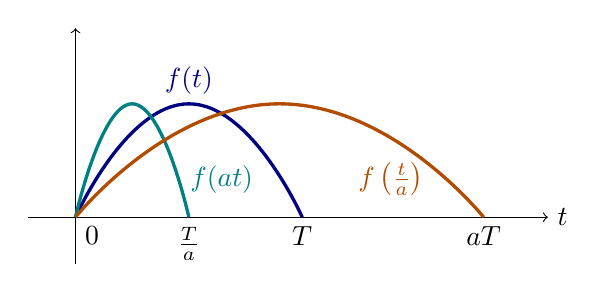
\begin{tikzpicture}[scale=1.2]
     	
     	\draw[->] (0,-0.5) -- (0,2);
     	\draw[->] (-0.5,0) -- (5,0) node[right] {$t$};
     	
     	
     	\draw[blue!50!black,very thick]
     	plot [smooth,tension=1] coordinates {(0,0) (1.2,1.2) (2.4,0)};
     	\draw (1.2,1.2) node[above,blue!50!black] {$f(t)$};
     	
     	\draw[blue!50!green,very thick]
     	plot [smooth,tension=1,xscale=0.5] coordinates {(0,0) (1.2,1.2) (2.4,0)};
     	\draw (1.2,0.4) node[right,xshift=-3,blue!50!green] {$f(at)$};
     	
     	\draw[green!30!red,very thick]
     	plot [smooth,tension=1,xscale=1.8] coordinates {(0,0) (1.2,1.2) (2.4,0)};
     	\draw (3.7,0.4) node[left,xshift=3,green!30!red] {$f\left(\frac{t}{a}\right)$};
     	
     	\draw (0,0) node[below right] {$0$};
     	
     	\draw (2.4,0) node[below] {$T$};
     	\draw (1.2,0) node[below] {$\frac{T}{a}$};
     	\draw (2.4*1.8,0) node[below] {$aT$};
     	\end{tikzpicture}
     \end{center}
     
     \paragraph{Τι συμβαίνει με τη συνέλιξη}
     \begin{align*}
     g(t) &= x(t)*h(t) \\
     x(t)&\to X(\omega )\\
     h(t)&\to H(\omega )\\
     y(t)&\to Y(\omega) = X(\omega)H(\omega)
     \end{align*}
     
     \begin{align*}
     y(t) &= x(t)\cdot h(t)\\
     y(t) &\to Y(\omega) = \frac{1}{2\pi}X(\omega)*H(\omega )
     \\ &= \frac{1}{2\pi} \int_{-\infty}^{\infty} X(\xi)H(\omega-\xi)\dif\xi
     \end{align*}
     
     \paragraph{}
     \begin{align*}
     f(t) &\to F(\omega)\\
     y(t)=\od{f(t)}{t}&\to j\omega F(\omega ) \\
     \od[n]{f(t)}{t}&\to (j\omega )^nF(\omega )
     \end{align*}
     \begin{align*}
     y(t)=\od{}{t}f(t) &= \od{}{t} \int_{-\infty}^{\infty} \frac{1}{2\pi}
     F(\omega ) e^{j\omega t}\dif \omega 
     \\ &= \frac{1}{2\pi}\int_{-\infty}^{\infty} F(\omega )\od{}{t}
     e^{j\omega t}]dif \omega 
     \\ &= \frac{1}{2\pi} \int_{-\infty}^{\infty} j\omega F(\omega )
     e^{j\omega t}\dif \omega 
     \end{align*}
     \subparagraph{}
     
     \begin{align*}
     f(t)&\to F(\omega )\\
     tf(t)&\xrightarrow{\text{F.T}}\od{}{t} F(\omega )\\
     t^nf(t)&\xrightarrow{\text{F.T}}\od[n]{}{t} F(\omega )\\
     \end{align*}
     
     \paragraph{}
     Φανταστείτε ότι \( f:\mathbb R\to\mathbb C \qquad 
     f(t) \xrightarrow F(\omega )
      \)
     
     \[
     f^*(t) \to F^*(-\omega )
     \]
     
     \begin{align*}
     f(t) &= \frac{1}{2\pi}\int_{-\infty}^{\infty} F(\omega)e^{j\omega t}\dif \omega \\
     f^*(t) &= \frac{1}{2\pi}\int_{-\infty}^{\infty} 
     F^*(\omega)e^{-j\omega t}\dif \omega \\
     &= \frac{1}{2\pi}\int_{-\infty}^{\infty}
     F^*(-\omega )e^{j\omega t}\dif \omega 
     \end{align*}
     
     \subsubsection{Θεώρημα Parseval}
     
     
     \begin{theorem*}[title=Θεώρημα Parseval,width=\textwidth]{Parseval}
        %TODO This doesn't look great
        \begin{align*}
        W = \int_{-\infty}^{\infty} \left| f(t) \right|^2\dif t
        =\frac{1}{2\pi}\int_{-\infty}^{\infty} \left|F(\omega )\right|^2
        \dif \omega = \int_{-\infty}^{\infty} A^2(\omega )\dif \omega 
        \end{align*}
        
        όπου \( \displaystyle F(\omega ) = A(\omega )e^{j\varPhi(\omega )} \)
     \end{theorem*}
     
     \begin{align*}
     y(t) &= f(t)f^*(t)=\left|f(t)\right|^2 \\
     Y(\omega ) &= \frac{1}{2\pi} F(\omega )*F^*(\omega ) \\
     Y(\omega ) &= \int_{-\infty}^{\infty} y(t)e^{-j\omega t}\dif t
     = \frac{1}{2\pi} \int_{-\infty}^{\infty} F(\xi) F^*\left(
     -(\omega -\xi) \right)\dif \xi
     = \frac{1}{2\pi}\int_{-\infty}^{\infty} \left|F(\omega )\right|^2\dif \omega 
     \\ &= \frac{1}{2\pi}\int_{-\infty}^{\infty} \left|A(\omega )\right|^2\dif\omega
     \end{align*}
     
     \begin{defn*}{}
        \textbf{Πυκνότητα φασματικής ενέργειας:}
        \(\displaystyle
        \frac{A(\omega)}{2\pi}
        \)
     \end{defn*}
     
     \subsubsection{Μετασχηματισμός Fourier γενικευμένων συναρτήσεων}
     \begin{enumgreekpar}
        \item\( \delta(t) \to 1 \)
        \[
        \int_{-\infty}^{\infty} \delta(t)e^{-j\omega t}\dif t=
        \left.e^{-j\omega t}\right|_{t=0}=e^0=1
        \]
        
        \( \delta(t\mp t_0) \to e^{\pm j\omega t_0} \)
        
        \( f(t) =1\to 2\pi\delta(\omega ) \), άρα
        \( \displaystyle \int_{-\infty}^{\infty}e^{-j\omega t }\dif t
        =2\pi\delta(\omega ) \implies \int_{-\infty}^{\infty} \cos\omega t \dif t
        -j\int_{-\infty}^{\infty}\sin\omega t\dif t = 2\pi\delta(\omega )\implies
        \begin{cases}
        \int_{-\infty}^{\infty} \cos\omega t\dif t = 2\pi\delta(\omega ) \\
        \int_{-\infty}^{\infty} \sin\omega t\dif t = 0
        \end{cases}
         \)
        
        \begin{tikzpicture}
        \draw (0,-1.5) -- (0,2);
        \draw[->] (-2,0) -- (2,0) node[below] {$t$};
        
        \draw[blue,ultra thick,->] (0,0) -- (0,1)
        node[right] {$\delta(t)$};
        
        \begin{scope}[xshift=5cm]
        \draw (0,-1.5) -- (0,2);
        \draw[->] (-2,0) -- (2,0) node[below] {$\omega$};
        
        \draw[blue,very thick] (-2,0.9) -- ++(4,0)
        node[midway,below right] {$1$};
        \filldraw[blue] (0,0.9) circle (0.7pt);
        \end{scope}
        \end{tikzpicture}
        
     \end{enumgreekpar}
     
     \subsubsection{}
     \[
     \mathrm{sgn}(t) = \frac{|t|}{t}
     \]
     
     \begin{tikzpicture}
     \draw[->] (0,-2) -- (0,2);
     \draw[->] (-2,0) -- (2,0) node[below] {$t$};
     
     \draw[ultra thick,blue] (-2,-1) -- ++(2,0) node[right] {$-1$};
     \draw[ultra thick,blue] (2,1) -- ++(-2,0) node[left] {$-1$};
     \end{tikzpicture}
     
     \begin{align*}
     \mathrm{sgn}(t)&=\lim_{u\to0}\left[
     e^{-a|t|}\mathrm{sgn}(t)
     \right] \\
     \mathrm{ FT }\ \mathrm{sgn}(t) &=
     \int_{-\infty}^{\infty} e^{-a|t|}\mathrm{sgn}te^{-j\omega t}\dif t
     \\ &= \lim_{a\to0}\int_{-\infty}^{0} e^{at-j\omega t}\dif t
     + \lim_{a\to 0} \int_0^\infty e^{-at-j\omega t}\dif t
     \\ &=
     \lim_{a\to0}\left[ \left.-\frac{e^{(at-j\omega t)}}{a-j\omega }
     \right|_{-\infty}^0 + \left. \frac{e^{-at-j\omega t}}{-(a+j\omega )}
     \right|_0^\infty
      \right]
     \\ &= \lim_{a\to 0} \left[ \frac{-1}{a-j\omega }+\frac{1}{a+j\omega} \right]
     \\ &= \frac{2}{j\omega }\in\mathbb I
     \end{align*}
     
     \paragraph{}
     \begin{align*}
     u(t) &\xrightarrow{\text{F.T.}} \\
     u(t) &= \frac{1}{2}+\frac{1}{2}\mathrm{sgn}(t)
     \xrightarrow{\text{F.T.}} \pi\delta(\omega ) +\frac{1}{j\omega }
     \end{align*}
     
     \begin{tikzpicture}
     \draw[->] (0,-1.5) -- (0,2) node[right] {$F(\omega)$};
     \draw[->] (-2,0) -- (2,0) node[below] {$\omega$};
     
     \draw[very thick,blue] plot [smooth,tension=1] coordinates {(-1.5,0) (0,1.2) (1.5,0)};
     
     \draw (1,-1) node[right] {$X(0) \to$ εκφράζει το D.C};
     \end{tikzpicture}
     
     \subsubsection{}     
     \begin{align*}
     \mathrm u(t) &\xrightarrow{\text{F.T.}} \pi\delta(\omega )+\frac{1}{j\omega }\\
     f(t) &\xrightarrow{\text{F.T.}} F(\omega ) \\
     g(t) &= \int_{-\infty}^{t}f(t)\dif t = \int_{-\infty}^{\infty} f(\tau)
     \mathrm u(t-\tau)\dif\tau = f(t)*\mathrm u(t) \\
     G(\omega ) &= F(\omega )\cdot\left[ \pi\delta(\omega )+\frac{1}{j\omega } \right]
     \end{align*}
     
     \subsubsection{}
     \begin{align*}
     \delta(t) &\to 1 \quad \text{άρτια} \\
     \delta^{(1)}(t)=\od{}{t}\delta(t) &\to j\omega \\
     \delta^{(n)}(t)=\od[n]{}{t}\delta(t) &\to (j\omega )^n
     \end{align*}
     \paragraph{}
     \begin{align*}
     t^n \to 2\pi j^n\delta^{(n)}(\omega )
     \end{align*}
     
     \subsubsection{}
     \paragraph{Παρ.}
     \begin{align*}
     f(t)&=|t| = t\mathrm u(t) - t\mathrm u(-t)\\
     F(\omega ) &= \frac{1}{2\pi}\left[
     2\pi j\delta(\omega )*\left[\pi\delta(\omega )+\frac{1}{j\omega }\right]
     -2\pi j \delta(\omega )*\left[ \pi\delta(\omega )-\frac{1}{j\omega } \right]
     \right]
     \end{align*}
     
     Calculate at home! The answer is \( -\frac{2}{\omega ^2} \)
     
     \begin{align*}
     t &\to 2\pi j^1\delta^{(1)}(\omega )\\
     \mathrm u(t) &\to \pi\delta(\omega )+\frac{1}{j\omega } \\
     \mathrm u(-t) &\to \pi\delta(\omega)-\frac{1}{j\omega }
     \end{align*}
     
     \subsubsection{Kramer's Kronig Relations}
     Από ηλεκτρομαγνητικό πεδίο: \[
       \underbrace{\vec D}_{\mathclap{\text{πυκνότητα ροής}}} = 
       \overbrace{\epsilon }^{\mathclap{\text{διηλεκτρική σταθερά}}}
       \underbrace{\vec E}_{\mathclap{\text{ένταση πεδίου}}}
     \]
     \begin{align*}
     \vec E =& \vec E(\vec r, t) \\
     &\vec E(\vec r,\omega ) \\
     \vec D(\omega ) =& \epsilon(\omega )\vec E(\omega )\\
     \vec D(t) =& \epsilon (t) +\vec E(t)
     \end{align*}
     
     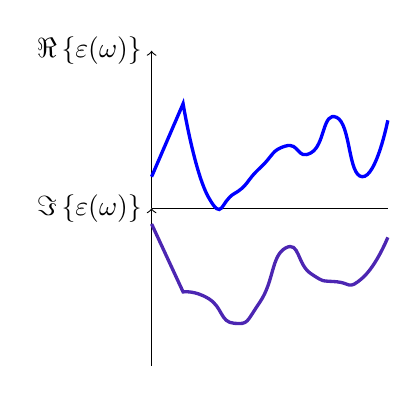
\begin{tikzpicture}
     \draw[->] (0,-2) -- (0,0) node[left]
     {$\Im\left\lbrace \varepsilon(\omega)\right\rbrace$};
     \draw[->] (0,0) -- (0,2) node[left]
     {$\Re\left\lbrace \varepsilon(\omega)\right\rbrace$};
     
     \draw (0,0) -- (3,0);
     
     \draw[very thick,blue] (0,0.4) --
     plot [smooth, tension=1, domain=0.4:3, samples=9] (\x,{0.8+0.7*rand});
     
     \draw[very thick,blue!70!orange] (0,-0.2) --
     plot [smooth, tension=1, domain=0.4:3, samples=9] (\x,{-0.8+0.7*rand});
     \end{tikzpicture}
     
     \paragraph{}
     \begin{align*}
     h(t) &= 0 \quad \forall t < 0 \\
     h(t)&: \mathbb R \to \mathbb R
     \end{align*}
    
    Αν \( H(\omega ) = \mathscr F T\left\lbrace h(t) \right\rbrace = H_R(\omega )
    +jH_I(\omega )
     \)
     
     \begin{align*}
     \Aboxed{ H_I(\omega ) &= -\frac{1}{\pi} \int_{-\infty}^{\infty}
     \frac{H_R(\omega)}{\omega -\omega'}\dif \omega ' } \\
     \Aboxed{ H_R(\omega ) &= \frac{1}{\pi} \int_{-\infty}^{\infty}
     \frac{H_I(\omega )}{\omega -\omega'}\dif \omega' }
     \end{align*}
     
     Η απόδειξη των σχέσεων θα πέσει στις εξετάσεις.
     
     \paragraph{Άσκ.}
     \begin{align*}
     f(t) &= 2\cos\omega_1 t \cos\omega_2 t = \cos(\omega_1-\omega_2)t
     +\cos(\omega_1+\omega_2)t
     \\ F(\omega ) &= \mathscr F\left\lbrace 
     \cos(\omega_1-\omega_2)t
      \right\rbrace + \mathscr F \left\lbrace \cos(\omega_1+\omega_2)t \right\rbrace
      \\ &=
      \pi \left[
      \delta\left( \omega -(\omega_1-\omega_2) \right)
      +\delta\left( \omega +(\omega_1-\omega_2) \right)
      \right] + \pi \left[
      \delta\left( \omega -(\omega_1+\omega_2) \right)
      +\delta\left( \omega +(\omega_1+\omega_2) \right)
      \right] 
     \end{align*}
     
     \( \left( \cos\omega_0t \xrightarrow{\text{FT}}
     \pi\left[ \delta(\omega -\omega_0)+\delta(\omega+\omega_0) \right]
      \right) \)
     
     Εναλλακτικά:
     \begin{align*}
     F(\omega ) &= 2\frac{1}{2\pi}\mathscr F \left\lbrace \cos\omega_1 t \right\rbrace
     * \mathscr F\left\lbrace \cos\omega_2 t \right\rbrace \\
     &= \pi \left[ \delta(\omega -\omega_1)+\delta(\omega+\omega_1) \right]
     * \left[ \delta(\omega -\omega_2)+\delta(\omega+\omega_2) \right]
     \\ &= \pi \left[
     \delta(\omega-\omega_2-\omega_1) +\delta(\omega-\omega_2+\omega_1)
     +\delta(\omega+\omega_2+\omega_1)+\delta(\omega+\omega_2-\omega_1)
     \right]
     \end{align*}
     
     \paragraph{Άσκηση}
     \begin{align*}
     f(t) &= g(t) \cos^2 \omega_0 t \qquad g(t) \xrightarrow{\text{FT}} G(\omega )
     \\ &= g(t)\frac{1+\cos2\omega_0 t}{2} = \frac{g(t)}{2} + 
     \frac{1}{2}g(t)\cos2\omega_0 t \\
     \implies F(\omega ) &= \frac{1}{2}G(\omega )+\frac{1}{2}G(\omega )
     *\mathscr F\left\lbrace \cos2\omega_0 t \right\rbrace
     \\ &= \frac{1}{2}G(\omega )+\frac{1}{2}G(\omega ) *
     \left[ \pi\left(\delta(\omega-2\omega_0)+\delta(\omega+2\omega_0)\right) \right]
     \frac{1}{2\pi} \\ &= \frac{1}{2}G(\omega ) + \frac{1}{4} \left[
     G(\omega -2\omega_0)+G(\omega +2\omega_0)
     \right]
     \end{align*}
     
     Αν δεν θυμάμαι τον τύπο:
     \begin{align*}
     f(t) &= g(t)\cos^2\omega_0 t = g(t)\cos\omega_0 t\cos\omega_0 t \\
     F(\omega ) &= \frac{1}{2\pi}G(\omega)*\left[
     \frac{1}{2\pi}\mathscr F\left\lbrace \cos\omega_0t \right\rbrace
     *\mathscr F \left\lbrace \cos\omega_0 t \right\rbrace
     \right] \\ &= \frac{1}{4\pi^2} G(\omega ) * \left[
     \pi\left[ \delta(\omega -\omega_1)+\delta(\omega+\omega_2) \right]
     \right] * \pi\left[
     \delta(\omega-\omega_1)+\delta(\omega+\omega_2)
     \right] \\ &=
     \frac{1}{4}G(\omega ) * \left[
     \delta(\omega -2\omega_0)+\delta(\omega)+\delta(\omega)+\delta(\omega+2\omega_0)
     \right]
     \\ &= \frac{1}{4}\left[
     G(\omega -2\omega_1)+2G(\omega )+G(\omega +2\omega_0)
     \right]
     \end{align*}
     
     \paragraph{Άσκηση}
     \begin{align*}
     f(t) &= g(at+b) \qquad g(t)\xrightarrow{\text{FT}}G(\omega ) \\
     h(t)=g(at) \qquad
     F(\omega ) &= \mathscr F\left\lbrace g(at)+b \right\rbrace
     = \mathscr F \left\lbrace h\left(t+\frac{b}{a}\right) \right\rbrace
     = H(\omega )e^{j\omega \frac{b}{a}} \\[5pt]
     H(\omega ) &= \frac{1}{|a|}G\left(\frac{\omega}{a}\right) \\
     \Aboxed{F(\omega ) &=
     \frac{1}{|a|}e^{j\omega\frac{b}{a}}G\left(\frac{\omega}{a}\right)}
     \end{align*}
     
     \paragraph{}
     \begin{align*}
     \cos t &\xrightarrow{\text{FT}} \pi\left[
     \delta(\omega -1)+\delta(\omega +1)
     \right] \\
     \sin \omega_0 t &= \cos\left(\omega_0t-\frac{\pi}{2}\right)
     \\
     \sin t &\xrightarrow{\text{FT}}
     \frac{1}{|\omega_0|}e^{-j\omega\frac{\pi}{2\omega_0}}\pi
     \left[ \delta\left(\frac{\omega}{\omega_0}-1\right)
     +\delta\left(\frac{\omega}{\omega_0} + 1\right)
      \right]
      \\ &\overset{\mathllap{\delta\left(\frac{\omega}{\omega_0}-1\right)
        = \delta\left(\frac{1}{\omega_0}(\omega-\omega_0)\right)}
        }{=}
        e^{-j\frac{\omega}{\omega_0}}\pi\left[
        \delta(\omega-\omega_0)+\delta(\omega +\omega_0)
        \right] \\ &= -j\pi\left[
        \delta(\omega -\omega_0)-\delta(\omega+\omega_0)
        \right]
     \end{align*}
     
     \paragraph{}
     \hspace{0pt}
     
     \begin{tikzpicture}
     \draw[->] (0,-1.5) -- (0,2) node[right] {$f(t)$};
     \draw[->] (-2,0) -- (2,0) node[below] {$t$};
     
     \draw[very thick,blue] (-1,0) -- ++(0,1) --++(2,0) -- ++(0,-1);
     \draw (0,1) node[above right] {$A$};
     
     \draw (-1,0) node[below] {$\sfrac{-\tau}{2}$};
     \draw (1,0) node[below] {$\sfrac{\tau}{2}$};
     
     \draw[<->] (-1,-0.6) -- ++(2,0) node[midway,below right] {$\tau$};

     \end{tikzpicture}
     
     \begin{align*}
     F(\omega ) &= \int_{-\infty}^{\infty} f(t)e^{-j\omega t}\dif t
     = A \int_{-\sfrac{\tau}{2} }^{\sfrac{\tau}{den} }e^{-j\omega t}\dif t
     \\ &= A\frac{1}{-j\omega }
     \left. e^{-j\omega t}\right|_{\sfrac{\tau}{2}}^{\sfrac{\tau}{2}}
     =\frac{A}{-j\omega }\left[ e^{-j\omega \sfrac{\tau}{2} } 
     -e^{j\omega \sfrac{\tau}{2}}
     \right] \\ &= A\tau\frac{\sin\left(\omega\frac{t}{2}\right)}{\frac{\omega t}{2}}
     \\ &= A\tau\frac{\sin\left(\frac{\omega t}{2}\right)}{\frac{\omega t}{2}}
     =A\tau \mathrm{sinc}\left(\frac{\omega t}{2\pi}\right)
     \end{align*}
     \begin{infobox}{sinc}
        \vspace{-5pt}
        \begin{align*}
        \text{Μαθηματικοί:}\quad \mathrm{sinc}(x)&=\frac{\sin x}{x}\\
        \text{Μηχανικοί:}\quad \mathrm{sinc}(x)&=\frac{\sin(\pi x)}{\pi x}
        \end{align*}
     \end{infobox}
     
     \subsection{Χρονοπερατό vs Ζωνοπερατό Σήμα}
     \begin{center}
     \begin{tikzpicture}
     \draw[->] (0,0) -- (0,2) node[right] {$f(t)$};
     \draw[->] (-3,0) -- (3,0) node[below] {$t$};
     
     \draw[very thick,blue] 
     plot[smooth] coordinates {(-2,0) (-1.9,0.5) (-1.7,0.7) (-1.5,0.4) (-1.2, 0.7)  
     	(-1, 0.9) (-0.8,0.1) (-0.5,0.5) (-0.3,0.5) (-0.1,0.7) (0,0.6) (0.1,0.8) (0.3,1.1)
     	(0.5,0.8) (0.6,0.9) (0.8,0.7) (1,0.5) (1.2,0.6) (1.5,0)
     } ;
     
     \draw (-2,0) node[below] {$A$};
     \draw (1.5,0) node[below] {$B$};
     
     \draw[<->] (-2,-0.5) -- ++(3.5,0) node[midway,below] {$T$};
     
     \draw (0,-1.2) node {$T$-timelimited};
     
     \begin{scope}[xshift=10cm]
     \draw[->] (0,-0.5) -- (0,2) node[right] {$G(\omega)$};
     \draw[->] (-2,0) -- (2,0) node[below] {$\omega$};
     
     \draw[very thick,blue] plot[smooth,tension=1.2] coordinates {(-1,0) (0,1) (1,0)};
     
     \draw (-1,0) node[below] {$\sfrac{-\sigma}{2}$};
     \draw (1,0) node[below] {$\sfrac{\sigma}{2}$};
     
     \draw (0,-1.2) node {$\sigma$-bandlimited};
     \end{scope}
     \end{tikzpicture}
     \end{center}
     
     \begin{itemize}
        \item Ένα ζωνοπερατό σήμα \textbf{δεν} μπορεί να είναι χρονοπερατό
        \item Ένα χρονοπερατό σήμα \textbf{δεν} μπορεί να είναι ζωνοπερατό
        \item Ένα σήμα μπορεί να μην είναι ούτε χρονοπερατό, ούτε ζωνοπερατό.
     \end{itemize}
     
     \begin{tikzpicture}
     \draw[gray,dashed] (-1,0) -- ++(0,-4);
     \draw[gray,dashed] (1,0) -- ++(0,-4);
     
     \draw[->] (0,-0.5) -- (0,2) node[right] {$f(t)$};
     \draw[->] (-2,0) -- (2,0) node[below] {$t$};
     
     \draw[very thick,blue] plot[smooth,tension=1.2] coordinates {(-1,0) (0,1) (1,0)};
     
     \draw (3,1) node {χρονοπερατό};
     
     \begin{scope}[yshift=-4cm]
     \draw[->] (0,-0.5) -- (0,2) node[right] {$f(t)$};
     \draw[->] (-2,0) -- (2,0) node[below] {$t$};
     
     \draw[very thick,blue] plot[smooth] 
     coordinates { (-2,-0.5) (-1,0) (0,1) (1,0) (2,-0.7)};
     
     \draw (3,1) node {ζωνοπερατό};
     
     \begin{scope}[xshift=6cm]
     \draw[->] (0,-0.5) -- (0,2) node[right] {$\hat f(\omega)$};
     \draw[->] (-2,0) -- (2,0) node[below] {$\omega$};
     
     \draw[very thick,blue] plot[smooth,tension=2] coordinates {(-1,0) (0,1.2) (1,0)};
     \end{scope}
     \end{scope}
     \end{tikzpicture}
     
     \paragraph{Απόδ.}
     \hspace{0pt}
     
   	\begin{tikzpicture}
   	\draw[->] (0,-0.5) -- (0,2) node[right,style={align=left}]
   	{Ζωνοπερατό\\$F(\omega)$};
   	\draw[->] (-2,0) -- (2,0) node[below] {$\omega$};
   	
   	\draw[very thick,blue] plot[smooth,tension=2] coordinates {(-1,0) (0,1.2) (1,0)};
   	
   	\draw (-1,0) node[below] {$\sfrac{-\sigma}{2}$};
   	\draw (1,0) node[below] {$\sfrac{\sigma}{2}$};
   	
   	\draw[->,thick] (2,1) -- ++(2,0) node[midway,above] {ΕΣΤΩ};
   	
   	\begin{scope}[xshift=6cm]
   	\draw[->] (0,-0.5) -- (0,2) node[right,style={align=left}]
   	{Χρονοπερατό\\$f(t)$};
   	\draw[->] (-2,0) -- (2,0) node[below] {$t$};
   	
   	\begin{scope}[xscale=1.3]
   	\draw[very thick,blue] plot[smooth,tension=1] coordinates {(-1,0) (0,1) (1,0)};
   	
   	\draw (-1,0) node[below] {$\sfrac{-T}{2}$};
   	\draw (1,0) node[below] {$\sfrac{T}{2}$};
   	\end{scope}
   	\end{scope}
   	
   	\end{tikzpicture}
     \begin{align*}
     f(t) &= \int_{-\sfrac{\sigma}{2} }^{\sfrac{\sigma}{2} } F(\omega )
     e^{j\omega t}\dif\omega \\
     \od[n]{f(t)}{t} &= \int_{-\sfrac{\sigma}{2} }^{\sfrac{\sigma}{2} }
     (j\omega )^n F(\omega )e^{j\omega t}\dif\omega
     \end{align*}
     Ορίζεται η σειρά Taylor επομένως σε οποιοδήποτε σημείο, όμως τότε, επειδή
     σε κάποια σημεία οι παράγωγοι είναι 0, θα έπρεπε η \( F \) να είναι
     μηδενική, άτοπο.
     
     \subsection{Γκαουσιανός παλμός}
     \[
     f(t) = \frac{1}{\sigma\sqrt{2\pi}}
     e^{\sfrac{t^2}{(2\sigma^2)} } \quad \xrightarrow{\quad\text{FT}\quad}
     F(\omega ) = e^{\frac{1}{2}\omega^2\sigma^2}
     = e^{-\frac{1}{2\frac{1}{\sigma^2}}\omega^2}
     \]
     
     \begin{center}
     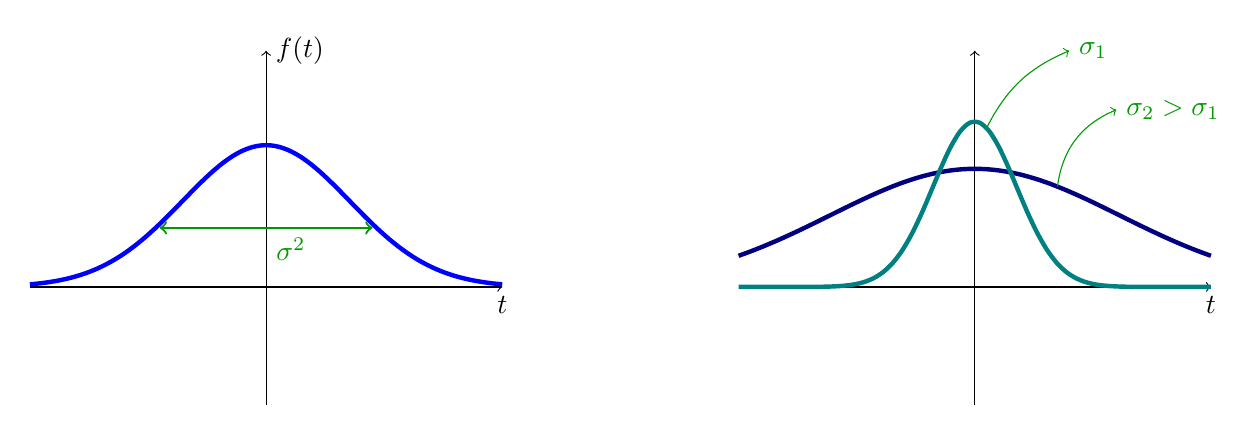
\begin{tikzpicture}[scale=1.5]
     \draw[->] (0,-1) -- (0,2) node[right] {$f(t)$};
     \draw[->] (-2,0) -- (2,0) node[below] {$t$};
     
     \draw[thick,green!60!black,<->] (-0.9,0.5) -- (0.9,0.5) node[below right,midway]
     {$\sigma^2$};
     
     \draw[ultra thick,samples=50,domain=-2:2,yscale=1.2,smooth,variable=\x,blue] 
     plot ({\x},{  exp(-\x*\x)  });
     
     \begin{scope}[xshift=6cm]
     \draw[->] (0,-1) -- (0,2);
     \draw[->] (-2,0) -- (2,0) node[below] {$t$};
     
     \draw[ultra thick,samples=50,domain=-2:2,yscale=1,smooth,variable=\x,blue!50!black] 
     plot ({\x},{  exp(-\x*\x/3)  });
     \draw[ultra thick,samples=50,domain=-2:2,yscale=1.4,smooth,variable=\x,
     blue!50!green] 
     plot ({\x},{  exp(-\x*\x*4)  });
     
     \draw[green!60!black,->] (0.1,{exp(-0.1^2*4)*1.4}) to[bend left=20] (0.8,2) node[right]
     {$\sigma_1$};
     \draw[green!60!black,->] (0.7,{exp(-0.7^2/3)}) to[bend left] (1.2,1.5) node[right]
     {$\sigma_2>\sigma_1$};
     \end{scope}

     \end{tikzpicture}
     \end{center}
     
     \begin{gather*}
     {\textstyle \int_{-\infty}^{\infty} f(t)\dif t = 1} \\
     \sigma^2 \text{ διασπορά}
     \end{gather*}
     \begin{align*}
     F(\omega ) &= \int_{-\infty}^{\infty} f(t)e^{-j\omega t}\dif t
     =\frac{1}{\sigma\sqrt{2\pi}}\int_{-\infty}^{\infty}
     e^{-\frac{t^2}{2\sigma^2}-j\omega t}\dif t
     \\ &= \frac{1}{\sigma\sqrt{2\pi}}\int_{-\infty}^{\infty}
     e^{-\frac{1}{\sigma^2}\left[
        t^2+2\sigma^2j\omega t+(j\omega \sigma^2)^2
        \right]}\cdot e^{\frac{1}{2\sigma^2}\left(j\omega \sigma^2\right)^2}\dif t
     \\ &=\frac{1}{\sigma\sqrt{2\pi}}e^{-\frac{1}{2\sigma^2}\omega^2\sigma^4}
     \int_{-\infty}^{\infty} e^{-\frac{1}{2\sigma^2} 
        \overbrace{\textstyle\left(t+j\omega\sigma^2\right)}^{t+j\omega\sigma^2-\tau}
        }\dif t
        \\ &= e^{-\frac{1}{2}\omega^2\sigma^2}\boxed{
            \frac{1}{\sigma\sqrt{2\pi}}\int_{-\infty}^{\infty}
            e^{-\frac{2}{\sigma^2}\tau^2}\dif\tau
            } = \displaystyle e^{\displaystyle -\frac{1}{2}\omega^2\sigma^2}
     \end{align*}
     
     Ηθικά διδάγματα:
     \begin{itemize}
        \item Ο μετασχηματισμός της Gaussian είναι Gaussian
        \item Ό,τι στενεύει στον χρόνο απλώνει στο φάσμα, και αντίθετα
     \end{itemize}
     \begin{center}
     		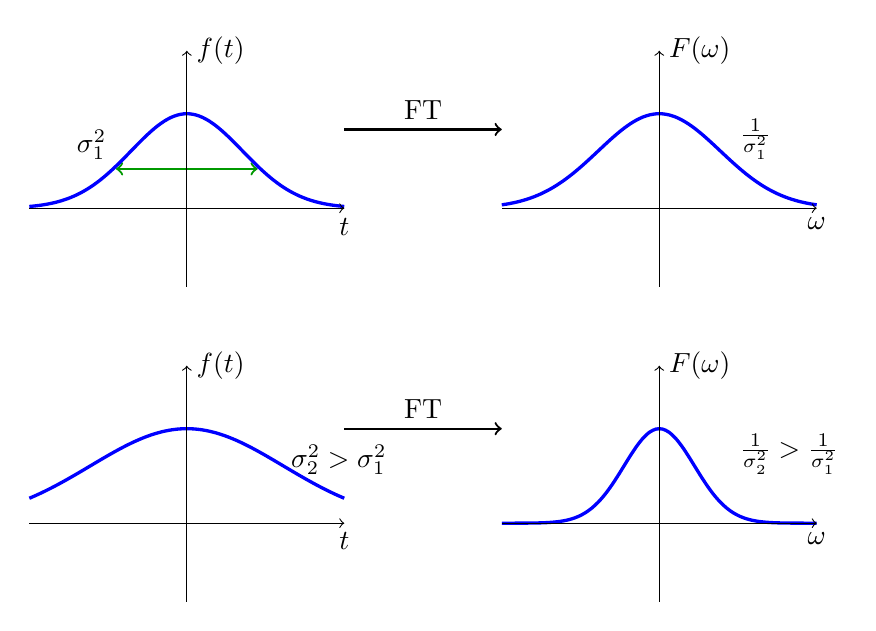
\begin{tikzpicture}
     		\draw[thick,green!60!black,<->] (-0.9,0.5) -- (0.9,0.5);
     		
     		\draw[very thick,samples=50,domain=-2:2,yscale=1.2,smooth,variable=\x,blue] 
     		plot ({\x},{  exp(-\x*\x)  });
     		
     		\draw[->] (0,-1) -- (0,2) node[right] {$f(t)$};
     		\draw[->] (-2,0) -- (2,0) node[below] {$t$};
     		
     		\draw (-0.9,0.5) node[above left,black] {$\sigma_1^2$};
     		
     		\draw[->,thick] (2,1) -- ++(2,0) node[midway,above] {FT};
     		
     		\begin{scope}[xshift=6cm]
     		
     		\draw[very thick,samples=50,domain=-2:2,yscale=1.2,smooth,variable=\x,blue] 
     		plot ({\x},{  exp(-\x*\x/1.2)  });
     		
     		\draw[->] (0,-1) -- (0,2) node[right] {$F(\omega)$};
     		\draw[->] (-2,0) -- (2,0) node[below] {$\omega$};
     		
     		\draw (0.9,0.5) node[above right,black] {$\frac{1}{\sigma_1^2}$};
     		\end{scope}
     		
     		\begin{scope}[yshift=-4cm]    
     		\draw[very thick,samples=50,domain=-2:2,yscale=1.2,smooth,variable=\x,blue] 
     		plot ({\x},{  exp(-\x*\x/3)  });
     		
     		\draw[->] (0,-1) -- (0,2) node[right] {$f(t)$};
     		\draw[->] (-2,0) -- (2,0) node[below] {$t$};
     		
     		\draw (1.2,0.5) node[above right,black] {$\sigma_2^2>\sigma_1^2$};
     		
     		\draw[->,thick] (2,1.2) -- ++(2,0) node[midway,above] {FT};
     		
     		\begin{scope}[xshift=6cm]
     		
     		\draw[very thick,samples=50,domain=-2:2,yscale=1.2,smooth,variable=\x,blue] 
     		plot ({\x},{  exp(-\x*\x/1.2*3)  });
     		
     		\draw[->] (0,-1) -- (0,2) node[right] {$F(\omega)$};
     		\draw[->] (-2,0) -- (2,0) node[below] {$\omega$};
     		
     		\draw (0.9,0.5) node[above right,black]
     		{$\frac{1}{\sigma_2^2} > \frac{1}{\sigma_1^2}$};
     		\end{scope}
     		\end{scope}
     		
     		\end{tikzpicture}
     \end{center}
     
     \paragraph{}
     \begin{gather*}
     \int_{-\infty}^{\infty} td^2(t)\dif t \\
     \text{διασπορά στον χρόνο} \quad d^2 = \int_{-\infty}^{\infty} t^2f^2(t)\dif t\\
     \text{διασπορά στο φάσμα}\quad D^2=\frac{1}{2\pi}
     \int\omega^2\left|\right|\dif\omega \\
     \left|\int_{-\infty}^{\infty} tx(t)\od{x(t)}{t}\dif t\right|
     \leq \int_{-\infty}^{\infty} t^2x^2(t)\dif t \cdot
     \int_{-\infty}^{\infty}\left|\od{x(t)}{t}\right|\dif t 
     \overset{\text{Parseval theorem}}{=} d^2D^2
     \implies \boxed{dD \geq \sfrac{1}{2} }
     \end{gather*}
     
     Γιατί \( \sfrac{1}{2}  \); (Υπόδειξη: \( 
     \int_{-\infty}^{\infty} tx\od{x}{t}\dif t =
     \int_{-\infty}^{\infty} t \frac{1}{2}\od{x^2}{t}\dif t
     = \left[ \quad \right] - \cancelto{1}{\frac{1}{2}\int x^2\dif t}
      \))
      
    Θα τα ξαναπούμε Τρίτη 22 Νοεμβρίου (χάνουμε 3 μαθήματα).
